\documentclass[a4paper]{article}

\usepackage[english]{babel}
\usepackage[utf8]{inputenc}
\usepackage{amsmath}
\usepackage{graphicx}
\usepackage{float}
\usepackage[colorinlistoftodos]{todonotes}

\title{Project: Leo Lani the talking robot}

\author{Selene Baez, Lenka Bajčetić and Bram Kraaijeveld \\
under the supervision of Piek van Vossen and Bob van Graft}

\date{\today}

\begin{document}
\maketitle

\begin{abstract}
During the academic year 2017-2018, we will work on an application to use a Pepper robot for communication. We aim to model Theory of mind and uncertainty while a one-on-one conversation occurs.
\end{abstract}

\newpage
\tableofcontents

\newpage
\section{Introduction}
\subsection{Vision}
\label{sec:vision}
The goal of this project is to create a system which allows Leo Lani, the VU Pepper robot, to have an informal conversation with an addressee. For this purpose, Leo Lani will not be presented as a know-it-all robot, but rather as an interactive talker and listener capable of "small talk" about various topics, as well as her surroundings. 

In order to go beyond stimulus-response tables, our goal is to create a system for purposeful speech which should be able to negotiate models during a conversation. This means the robot will have both her and her speaker's theory of mind ,and the awareness they might not be the same. 

Furthermore, Leo Lani will be able to remember when she has met a person before, along with some information mentioned in previous conversations, as well as a model of a current conversation. When talking to a famous person, she will recognize him/her as such and gather basic information related to them. 

Finally, Leo Lani should lead a conversation as naturally as possible, and this includes generating and detecting non-verbal cues, such as a pointing finger or nodding. All of these tasks are important for Leo Lani to be capable to lead a conversation, but they are all quite complex to implement. This is why an initial model needs to be planned. This model would have limited functionalities but allow for easy upgrades while the project is progressing. 

\subsection{Desired behavior}
The conversation should not be restricted by the topics, so the model needs some way to handle open domain. The idea is to recognize key words and try to steer the conversation into a familiar topic. If there are no recognized entities Leo Lani should ask a question on a different topic.

The entities recognized do not need to be an exact match from a dictionary, in case of uncertainty (which comes in any case with speech-to-text transcription) the system should ask for clarification. As such, the system should be able to have a dialogue about one of the topics but handle input from open domain. In order to lead a conversation the system needs to handle co-reference and have a way to connect previously mentioned entities. 

Lastly, in order to make Leo Lani more "aware", it is our goal to implement a visual detection system which would run in parallel to the dialog system. The visual detection system would recognize prominent surrounding objects, so these could be another topic of conversation. This way we would attempt to make a model which solves the symbol grounding problem, and gives Leo Lani the capability of situated language. 

\subsection{Project overview}
This project consists of modules orchestrated together to achieved the described desired behavior. 


\newpage
\section{Sensory mechanisms}

\subsection{Speech recognition}
We rely on Google Speech to recognize natural English language. This service performs some curation on the recognized speech, but ideally our the conversation context will aid in extra processing of the output.

Since our goal relies heavily on identifying people, the speech recognition module should specialize in recognizing names. For this purpose, we utilize Google Speech on different Languages, to get the most likely text matching the speech detected. In case of failure to recognize a name, the alternatives are to speel a name or input the name in the tablet. 

\subsection{Face recognition}
OpenFace provides with a package for Face Recognition. It generates a 128-dimensional vector representing a face. 

\subsubsection{Gender recognition}

\subsection{Speech production}
% Body language
For now, we use the built in Pepper voice. In the future, we will most likely use Watson Text to Speech in order to accommodate different languages.

\newpage
\section{Knowledge representation}

\subsection{Factual knowledge}
Some general factual knowledge can be accessed by Leo Lani by means of external databases. An example is using \textbf{Wolfram alpha}

\subsection{Conversation topics}
Here we gather knowledge regarding general topics recurrent in small talk. Some candidates are: 

\begin{itemize}
\item The weather: Current state of weather, how will the weather be on the weekend, etc
\item Railway and public transit in general: Common complaints about transit, delays, etc
\item Sports: Discuss about "last night's game", the Champions League, or women soccer
\item AI in pop culture: Comment on common views about robotics and Artificial Intelligence. 
\item News: Information about current events in some domain
\end{itemize}

These topics require different information and a different approach. Transport, sports, news and weather talk would need daily updates and a certain tone, e.g. complaining or being optimistic about nice weather. Talking about AI would require answering more insightful questions and either needs a very advanced NLU system, or a set of hard-coded answers (at least for questions about awareness, ethical questions, etc.) Another possible approach would be to try to make a vocabulary of definitions for these concepts and give simple answers. The ultimate goal would be to have a system capable of asking questions about things it does not recognize as well. It would also be good to pair this knowledge with some more contextual information, ideally visual as well. 

We can access existing knowledge bases related to this topics. \textbf{Dbpedia} could be a good starting point for this. 


\subsection{Memory}
The robot should remember people who it has talked to before. There also needs to be some sort of first-level memory for the current conversation.

% Privacy
\subsubsection{Ontology}
We can create an ontology (similar to FOAF) regarding people and their basic information (place of origin, interests, place of work, etc). This will be uploaded to a triple store and filled in as the robot has different  conversations. This information paired with entries from DBpedia can be a good source for initiating conversations. 

As a further step, the robot can reason over the ontology in order to find people who could potentially know each other. For example, people from the same country, smae department, or with the same interests. 

\begin{figure}[h]
  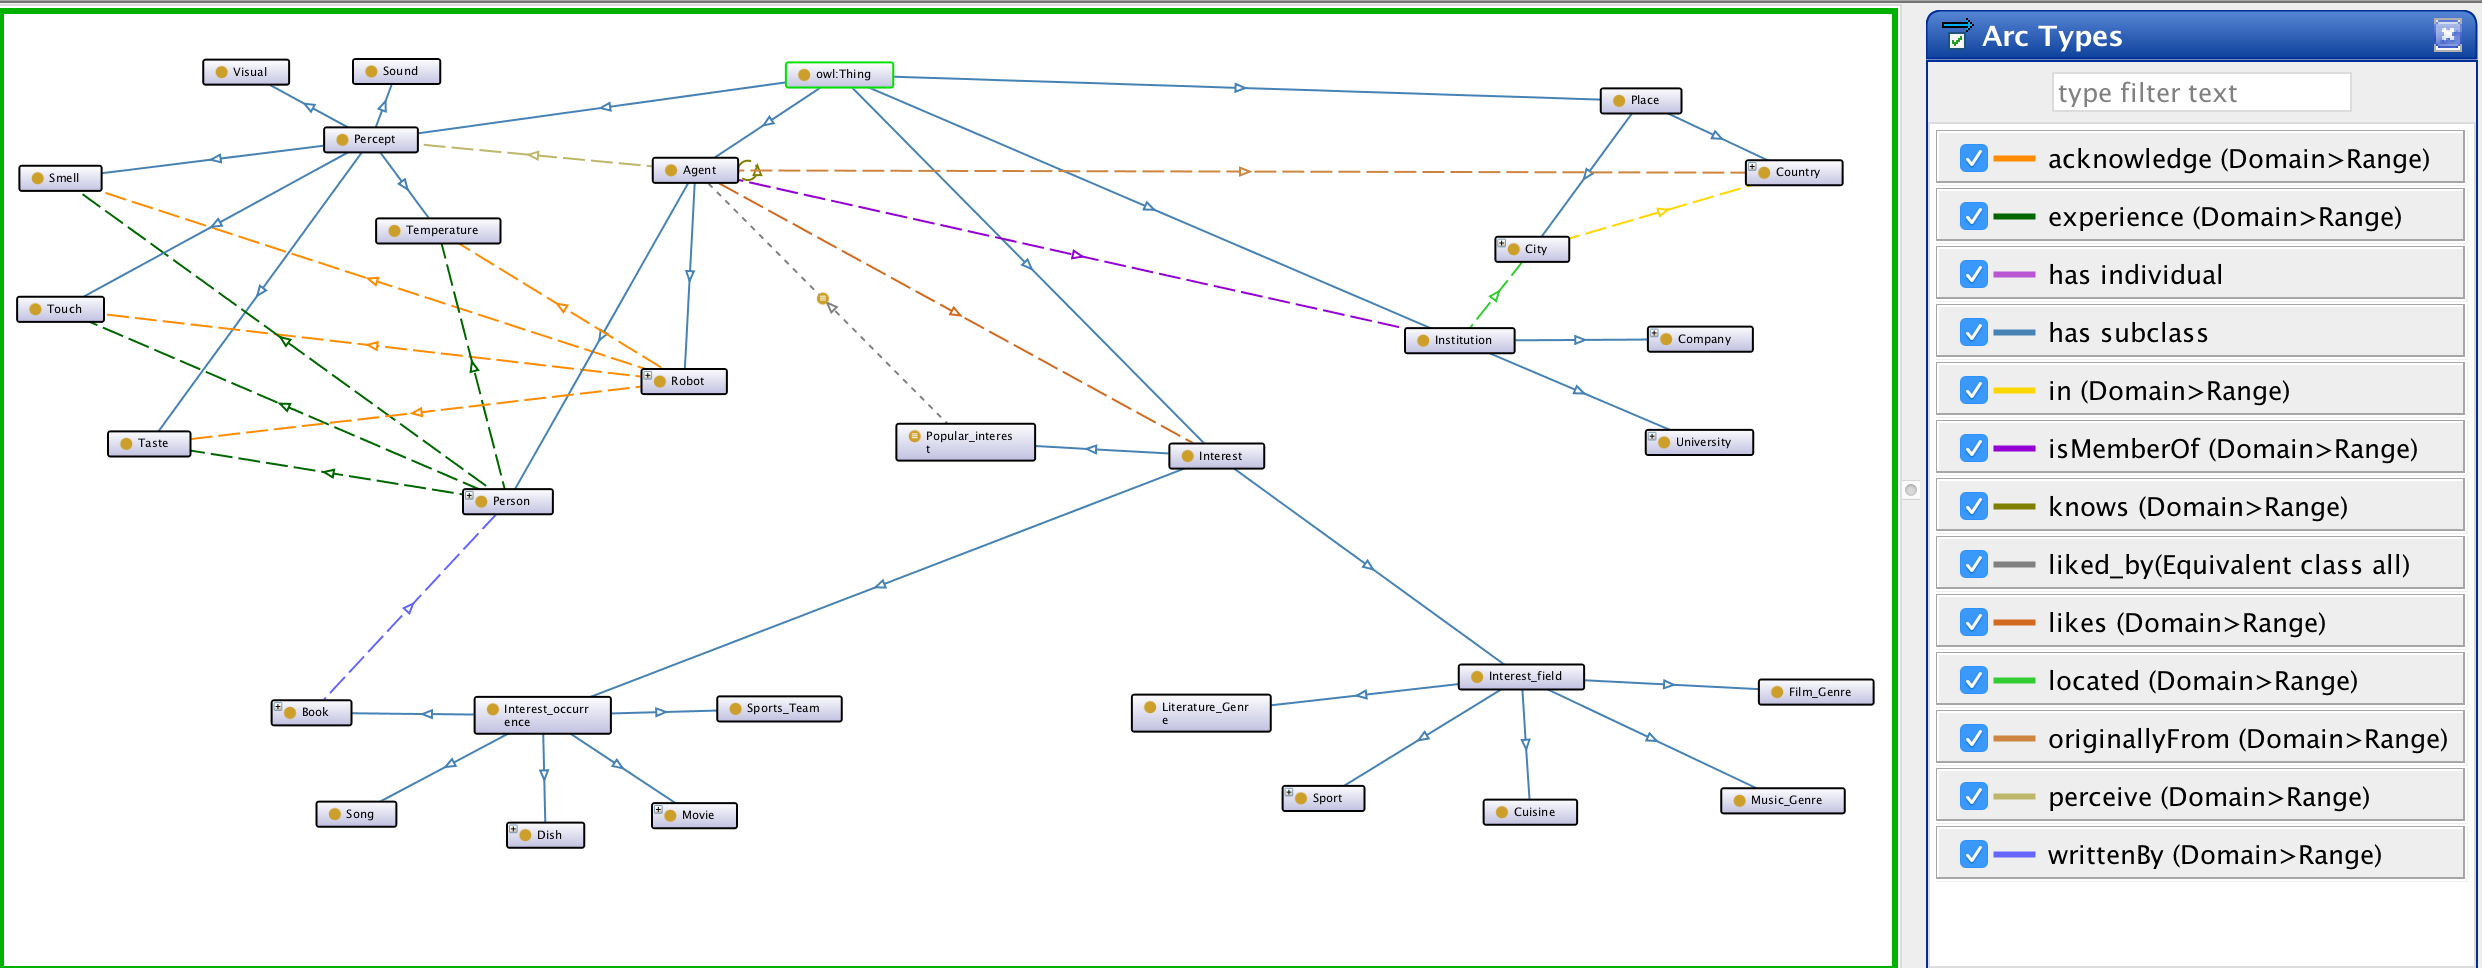
\includegraphics[width=\linewidth]{images/ontology.png}
  \caption{Ontology.}
  \label{fig:ontology}
\end{figure}

\subsubsection{Triple store and queries}


\newpage
\section{Models}

\subsection{Theory of mind}
Having memory involves storing information about the world. Yet, some memories can be conflicting. We as humans, are familiar with this notion and resolve conflicts as we go. Furthermore, while having a one-on-one conversation we need to recognize that what "I know" is a perspective and can be uncertain. Thus, this project attempts to model both the speaker and the addressee's theory of mind, what they think and what they think the other might think. 

For Leo Lani, we have created a model that stores information in terms of triples, or statements. However, we have not yet modeled a mechanism to model and possibly resolve uncertainty. 

\textbf{GRaSP} allows to add information to knowledge, such as provenance (who said it, where I read it, how do I know this). 

Furthermore, by gathering this information we can score statements 

\subsection{Conversation flow}
In order to guide and respond during the conversation, Leo Lani needs to reason over her knowledge (about herself, the addressee and the world) while taking into account her goals for the interaction. 

\subsubsection{BDI model}
BDI models (Beliefs, Desires, and Intentions)

\begin{figure}[h]
  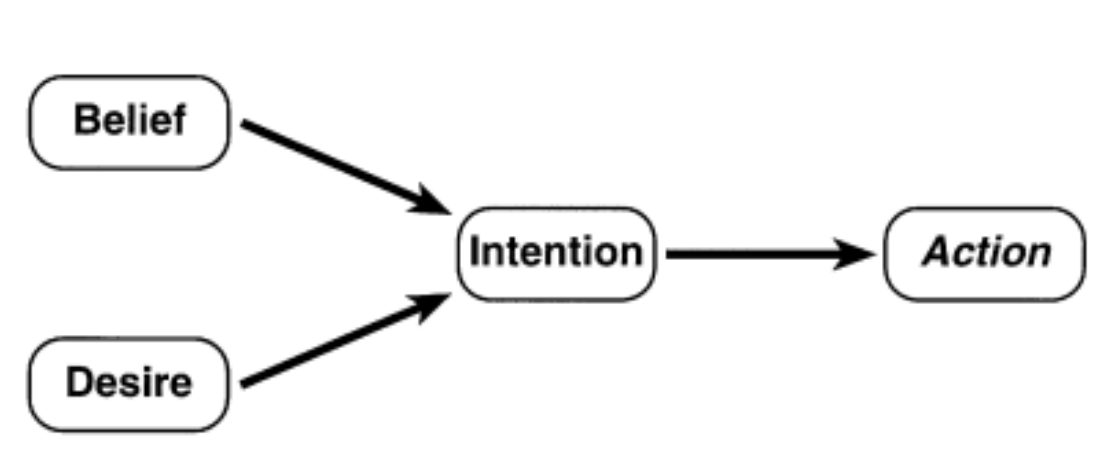
\includegraphics[width=\linewidth]{images/BDI.png}
  \caption{BDI model.}
  \label{fig:BDI model}
\end{figure}

In summary, we can define a BDI agent by specifying its knowledge base and its plan library. 

\begin{table}[h]
\centering
\begin{tabular}{||c|p{2.5cm}|p{2.5cm}|p{2.5cm}||}
\hline
\textbf{Agent} & \textbf{Desires} & \textbf{Beliefs} & \textbf{Intentions} \\
[0.5ex] 
\hline \hline
Leo lani & 
Gather information about the speaker or the world & 
Information about context (date, time, location) &  \\
& Social talk regarding a topic & Information about the person speaking &  \\
& & Information about the conversation topic &  \\
& & Information extracted from current conversation & \\
\hline
Addressee &  &  &  \\ [1ex]
\hline 
\end{tabular}
\caption{BDI model for this application}
\label{table:BDI}
\end{table}

\subsubsection{Reasoning}

\begin{figure}[H]
  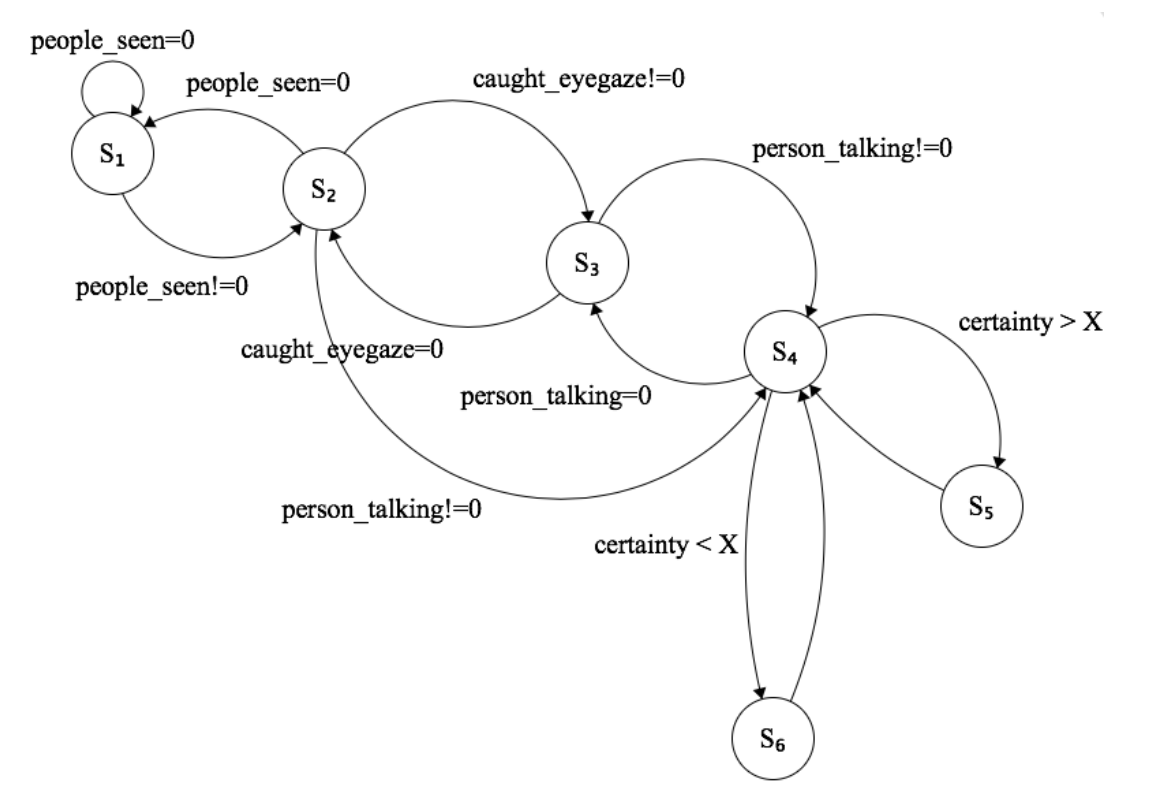
\includegraphics[width=\linewidth]{images/FSM.png}
  \caption{Finite state machine representing Leo Lani's reasoning while having a conversation.}
  \label{fig:FSM}
\end{figure}

\subsection{Robot personality}
The robot could also potentially develop its own personality during the conversation. It could show it is bored when it is not interested in a specific topic, confused when it is asked many questions at the same time, nervous when talking in public, or others. 

\textbf{Tool: BDI-M extension?}
We can extend the BDI model to include Mood. This extension would allows us to model the addressee's mood (through the built it detectors and Watson detector), and also model Leo Lani's own mood. 

\subsection{Opinions}
Speech acts verbs: cognitive verbs (emotion, opinion)
% Opinion mining out of the box



\newpage

\section{Planning and division of work}

As mentioned, since the vision is both broad and deep, there needs to be an incremental approach with an ordered list of priorities. Currently, Leo Lani has a text-to-speech and a speech-to-text module, as well as object detection. This is already a good start. Some of the next steps can be:
\begin{itemize}
\item Designing an ontology
\item Designing a theory of mind for Leo Lani and for Leo Lani's conversational partner
\item Design a model for handling open-domain talk (can be very simple at first)
\item Find a way to connect sensory information to symbolic representation
\item Create a system for handling uncertainty through asking confirmation
\item Create a human database and a system for people recognition 
\item Create a model for non-verbal communication

% Facebook, Blog

\end{itemize}
\begin{table}[h]
\centering
\begin{tabular}{|l|l|r|}
Phase & Deadline & Person in charge \\\hline
Planning and delimitation & Nov 3rd & Everyone  \\
Design architecture & Nov 10th & Everyone \\
BDI & Nov 17th & \\
Topic ontology (Sports) & Nov 24th & \\
Theory of mind (goal: validate knowledge) & Dec 1st & Bram, Lenka, Selene \\ 
Industry market & Dec 8th & Everyone \\
Person ontology & & \\
Memory & & \\
Speech production/recognition & & \\
Workshop with UvA & Spring &  Everyone \\
Opening of the new building & 2018 & Everyone \\
\end{tabular}
\caption{\label{tab:planning} Planning.}
\end{table}

\newpage

\begin{thebibliography}{9}
\bibitem{nano3}
Nikolaos Mavridis, \emph{A review of verbal and non-verbal human–robot interactive communication}. Interactive Robots and Media Lab, Agia Paraskevi, Athens
\end{thebibliography}
\end{document}